\documentclass[11pt,a4paper]{article}
\usepackage[T1]{fontenc}
\usepackage[margin=2.3cm]{geometry}
\usepackage{amsmath,amssymb}
\usepackage{graphicx}
\usepackage[dvipsnames]{xcolor}
\usepackage{enumitem}
\usepackage[colorlinks=true,linkcolor=blue,urlcolor=blue]{hyperref}
\setlength{\parskip}{0.6em}
\setlength{\parindent}{0pt}
\begin{document}

\begin{center}{\LARGE\bfseries opencollisions}\\[0.4em]{\large Predict what happens in collisions with momentum and energy, in three sessions.}\\[0.2em]\small PAN IIT OSS explainer \textbullet{} secondary to diploma/undergrad (levels 3-5)\end{center}

\section*{Why this exists}
Collisions are everywhere: a cue ball, a car crash, a bullet in a block, a ball bouncing on a floor. This explainer shows the mathematics behind them: two conservation laws, one number for bounciness and a simulation that checks the formulas.

\section*{The end goal}
The end goal is to predict what happens in collisions with momentum and energy. The same ideas carry over to particle physics, to sports and to vehicle safety, with more bodies, rotation and breaking materials.

\section*{How the three sessions build up}
\begin{enumerate}[nosep]
\item \textbf{Session 1: Momentum is kept, energy may not be: sticking and bouncing} (Level 1: conceptual interactive model, 60 min).
\item \textbf{Session 2: Every collision in between: restitution, energy lost and the ballistic pendulum} (Level 2: mathematical engineering model, 75 min).
\item \textbf{Session 3: Off-centre hits: discs in two dimensions, a contact simulation and a crash estimate} (Level 3: simulation and validation, 90 min).
\end{enumerate}

\section{Session 1: Momentum is kept, energy may not be: sticking and bouncing}

\subsection*{A. Real-world problem}
Two carts roll toward each other on a smooth track. In one collision they stick together, in another they bounce apart. What happens to their speeds afterwards, and what is the same in both collisions? Where does the kinetic energy go when the carts stick?

\subsection*{B. Concept and theory}
Choose one direction as positive; a body moving the other way has a negative speed. The momentum of a body is p = m v and its kinetic energy is KE = 1/2 m v\textasciicircum{}2. During the short collision the two bodies push on each other with equal and opposite forces for the same time, so the momentum one gains the other loses: the total momentum of the pair is the same before and after. In a sticking collision (perfectly inelastic) the bodies leave together, v = (m1 v1 + m2 v2) / (m1 + m2), and some kinetic energy is turned into heat, sound and deformation. In a perfectly bouncing collision (perfectly elastic) the kinetic energy is also kept; together with momentum this gives v1' = ((m1 - m2) v1 + 2 m2 v2) / (m1 + m2) and v2' = ((m2 - m1) v2 + 2 m1 v1) / (m1 + m2). Real collisions lie between the two. Momentum is conserved in all of them, as long as no outside force acts during the collision.

\begin{itemize}[nosep]
\item m1, m2: masses of the two bodies (kg)
\item v1, v2: speeds before the collision (negative if moving in the negative direction) (m/s)
\item v1', v2': speeds after a bouncing collision (m/s)
\item v: common speed after a sticking collision (m/s)
\item p: momentum, m v (kg m/s)
\item KE: kinetic energy, 1/2 m v\textasciicircum{}2 (J)
\end{itemize}

\[ p = m v,\qquad KE = \tfrac{1}{2} m v^{2},\qquad m_1 v_1 + m_2 v_2 = m_1 v_1' + m_2 v_2' \]

\[ v = \frac{m_1 v_1 + m_2 v_2}{m_1 + m_2}\ \text{(sticking)} \]

\[ v_1' = \frac{(m_1 - m_2) v_1 + 2 m_2 v_2}{m_1 + m_2},\qquad v_2' = \frac{(m_2 - m_1) v_2 + 2 m_1 v_1}{m_1 + m_2}\ \text{(bouncing)} \]

\subsection*{C. Visual explanation}
The first figure compares three states of the same collision: the momentum is identical before, after sticking and after bouncing, but the kinetic energy only stays the same after bouncing. The second figure plots the speeds after the collision against the mass ratio m2 / m1 for a body 1 of 1 kg moving at 4 m/s and a body 2 at rest: for a heavy target (large ratio) body 1 bounces back with a negative speed, and for equal masses it stops.

\begin{figure}[h]\centering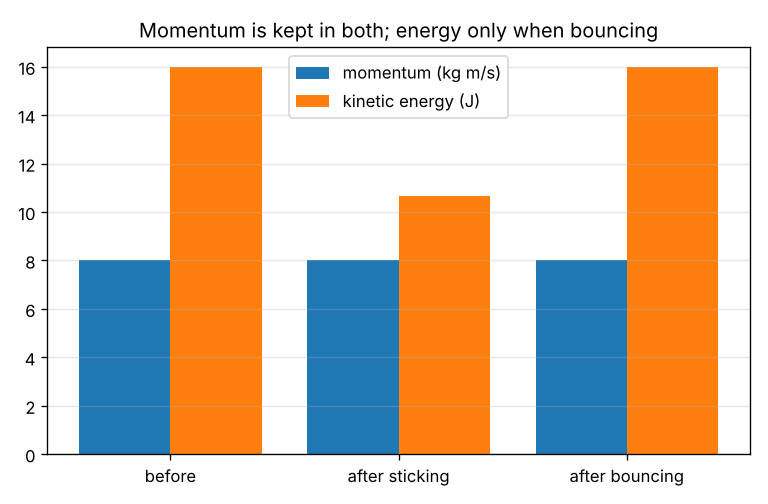
\includegraphics[width=0.78\textwidth]{figures/s01_conserved.png}\caption{Momentum and kinetic energy before, after sticking and after bouncing.}\end{figure}

\begin{figure}[h]\centering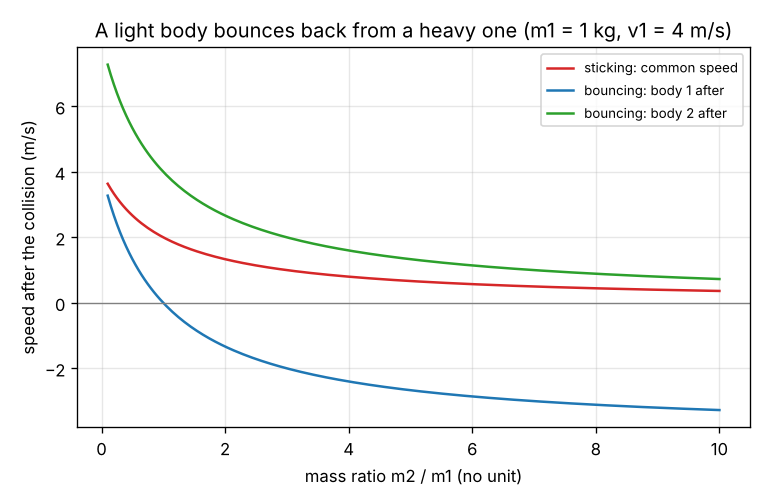
\includegraphics[width=0.78\textwidth]{figures/s01_speeds_vs_mass_ratio.png}\caption{Speeds after the collision against the mass ratio m2 / m1.}\end{figure}

\subsection*{E. Worked example}
\textbf{Problem.} A 2 kg cart moving at 4 m/s hits a 1 kg cart at rest. Find the speeds if they stick, and if they bounce perfectly. In each case, check the momentum and find the kinetic energy lost.

\begin{enumerate}[nosep]
\item Before: p = 2 x 4 + 1 x 0 = 8 kg m/s and KE = 1/2 x 2 x 16 = 16 J.
\item Sticking: v = 8 / 3 = 2.667 m/s. After: KE = 1/2 x 3 x 2.667\textasciicircum{}2 = 10.67 J, so 5.33 J are lost (one third).
\item Bouncing: v1' = (2 - 1) x 4 / 3 = 1.333 m/s and v2' = 2 x 2 x 4 / 3 = 5.333 m/s.
\item Check momentum: 2 x 1.333 + 1 x 5.333 = 8.00 kg m/s.
\item Check energy: 1/2 x 2 x 1.333\textasciicircum{}2 + 1/2 x 1 x 5.333\textasciicircum{}2 = 16.00 J, equal to the 16 J before.
\end{enumerate}
\textbf{Answer.} Sticking: 2.667 m/s and 5.33 J lost. Bouncing: 1.333 m/s and 5.333 m/s, with no energy lost. Momentum is 8 kg m/s in both.

\section{Session 2: Every collision in between: restitution, energy lost and the ballistic pendulum}

\subsection*{A. Real-world problem}
A basketball dropped from 1 m comes back to 0.64 m. A bullet buried in a hanging block makes it swing up a few centimetres. What happens in collisions that are neither perfectly sticky nor perfectly bouncy, how much energy disappears, and how can a swing tell us the speed of a bullet that is far too fast to time?

\subsection*{B. Concept and theory}
The speed of separation after a collision is a fixed fraction of the speed of approach before it: e = (v2' - v1') / (v1 - v2), with e between 0 and 1. For e = 1 the collision is perfectly bouncing, for e = 0 it is sticking. Together with momentum conservation, this gives v1' = (m1 v1 + m2 v2 + m2 e (v2 - v1)) / (m1 + m2) and v2' = (m1 v1 + m2 v2 + m1 e (v1 - v2)) / (m1 + m2). The kinetic energy that is lost depends on the reduced mass mu = m1 m2 / (m1 + m2): dKE = 1/2 mu (1 - e\textasciicircum{}2) (v1 - v2)\textasciicircum{}2. A ball dropped from a height h reaches the floor with speed sqrt(2 g h) and leaves with sqrt(2 g h'), so e = sqrt(h' / h). In a ballistic pendulum the bullet sticks in the block (momentum is kept, e = 0), and the swing then converts kinetic energy into height: v\_bullet = (m + M) / m x sqrt(2 g h). e cannot be above 1 (that would create energy) or below 0 (the bodies would pass through each other).

\begin{itemize}[nosep]
\item e: coefficient of restitution (no unit)
\item mu: reduced mass, m1 m2 / (m1 + m2) (kg)
\item dKE: kinetic energy lost in the collision (J)
\item h, h': drop height and rebound height (m)
\item m, M: bullet mass and block mass (kg)
\item g: gravitational acceleration (m/s\textasciicircum{}2 (9.81))
\end{itemize}

\[ e = \frac{v_2' - v_1'}{v_1 - v_2},\qquad 0 \le e \le 1 \]

\[ v_1' = \frac{m_1 v_1 + m_2 v_2 + m_2 e (v_2 - v_1)}{m_1 + m_2},\qquad v_2' = \frac{m_1 v_1 + m_2 v_2 + m_1 e (v_1 - v_2)}{m_1 + m_2} \]

\[ \Delta KE = \tfrac{1}{2}\mu (1 - e^{2})(v_1 - v_2)^{2},\qquad e = \sqrt{h'/h},\qquad v_{\mathrm{bullet}} = \frac{m + M}{m}\sqrt{2 g h} \]

\subsection*{C. Visual explanation}
The first figure plots the two speeds after the collision against e for a 2 kg body at 4 m/s hitting a 1 kg body at -1 m/s. At e = 0 the lines meet at the common speed of the sticking collision, and as e grows they spread apart: the speed of separation is e times the speed of approach. The second figure plots the kinetic energy lost: it is largest at e = 0 and falls to zero at e = 1, following the curve 1 - e\textasciicircum{}2.

\begin{figure}[h]\centering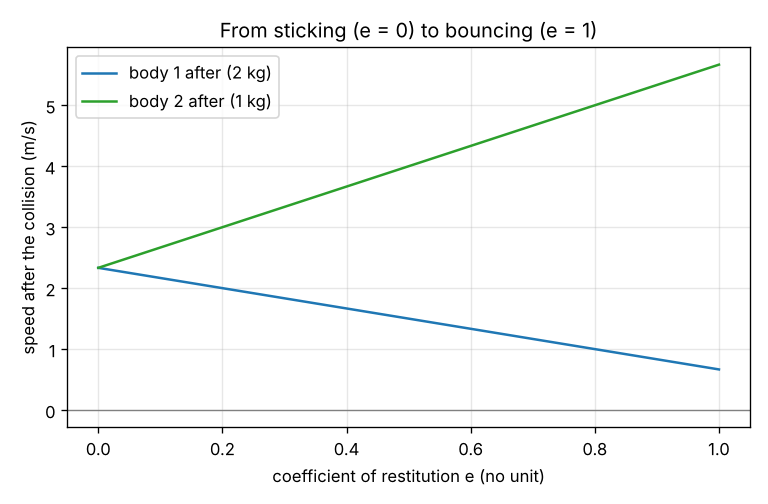
\includegraphics[width=0.78\textwidth]{figures/s02_speeds_vs_e.png}\caption{Speeds after the collision against the coefficient of restitution.}\end{figure}

\begin{figure}[h]\centering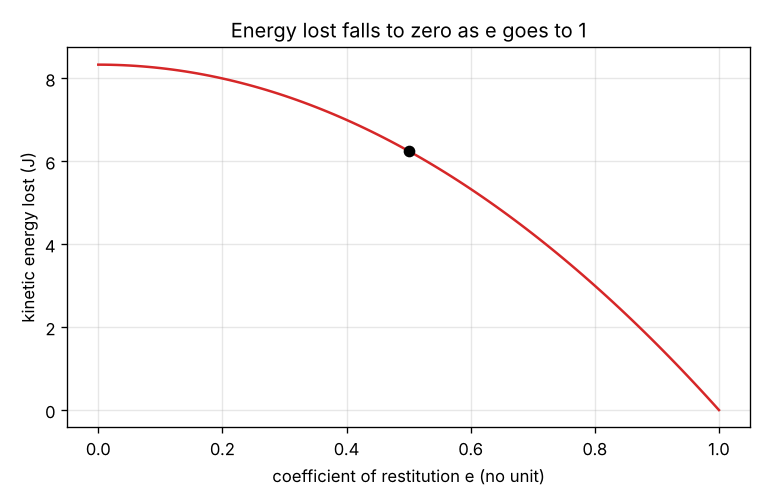
\includegraphics[width=0.78\textwidth]{figures/s02_energy_lost_vs_e.png}\caption{Kinetic energy lost against e; the dot is the worked example (e = 0.5).}\end{figure}

\subsection*{E. Worked example}
\textbf{Problem.} A 2 kg body moving at 4 m/s hits a 1 kg body moving at -1 m/s (towards it). The coefficient of restitution is e = 0.5. Find both final speeds and the kinetic energy lost.

\begin{enumerate}[nosep]
\item Momentum before: 2 x 4 + 1 x (-1) = 7 kg m/s. The speed of approach is 4 - (-1) = 5 m/s.
\item v1' = (7 + 1 x 0.5 x (-1 - 4)) / 3 = (7 - 2.5) / 3 = 1.50 m/s.
\item v2' = (7 + 2 x 0.5 x (4 + 1)) / 3 = (7 + 5) / 3 = 4.00 m/s. Check: the speed of separation is 4.00 - 1.50 = 2.50 = 0.5 x 5 = 2.5.
\item Momentum after: 2 x 1.50 + 1 x 4.00 = 7.00 kg m/s.
\item Kinetic energy: before 1/2 x 2 x 16 + 1/2 x 1 x 1 = 16.50 J, after 1/2 x 2 x 2.25 + 1/2 x 1 x 16 = 10.25 J.
\item Lost: 16.50 - 10.25 = 6.25 J. Check with the formula: mu = 2/3, so 1/2 x 2/3 x (1 - 0.25) x 25 = 6.25 J.
\end{enumerate}
\textbf{Answer.} v1' = 1.50 m/s, v2' = 4.00 m/s, and 6.25 J of kinetic energy are lost.

\section{Session 3: Off-centre hits: discs in two dimensions, a contact simulation and a crash estimate}

\subsection*{A. Real-world problem}
Two billiard balls hit off-centre: the first is deflected and the second leaves at an angle. How do the speeds and angles depend on how far off-centre the hit is, and can we trust the formulas? Then the same ideas on a larger scale: a car hits a wall, and the front crumples over a short distance. How large are the average force and the deceleration, and what must a designer change to keep them below a limit?

\subsection*{B. Concept and theory}
Disc 1 moves along +x. Disc 2 sits a distance b (the impact parameter) above that line. At contact the line from the centre of disc 1 to the centre of disc 2 makes an angle phi with sin(phi) = b / (R1 + R2); call its unit vector n. Smooth discs push on each other only along n, so only the component of the relative velocity along n changes: with v\_n = (v1 - v2) . n, v1' = v1 - m2 / (m1 + m2) (1 + e) v\_n n and v2' = v2 + m1 / (m1 + m2) (1 + e) v\_n n. The component across n does not change. The kinetic energy lost is 1/2 mu (1 - e\textasciicircum{}2) v\_n\textasciicircum{}2. For equal masses, e = 1 and v2 = 0, momentum and energy conservation make the two outgoing velocities perpendicular. As an independent check, we let the discs overlap slightly and push each other with a stiff spring (force k x overlap along n) and a damper whose damping ratio gives the chosen e, and step the motion forward in small time steps; the final velocities must agree with the formula. For the car, the work done by the average crumple force over the crumple distance d equals the initial kinetic energy: F d = 1/2 m v\textasciicircum{}2, so the average deceleration is a = v\textasciicircum{}2 / (2 d).

\begin{itemize}[nosep]
\item b: impact parameter: offset of disc 2 from the line of motion of disc 1 (m)
\item R1, R2: radii of the discs (m)
\item phi: angle of the line of centres at contact, sin(phi) = b / (R1 + R2) (degrees)
\item n: unit vector from the centre of disc 1 to the centre of disc 2 (no unit)
\item v\_n: component of the relative velocity along n (m/s)
\item k: contact spring stiffness (simulation) (N/m)
\item F, a: average crumple force and average deceleration (N, m/s\textasciicircum{}2)
\item d: crumple distance (m)
\end{itemize}

\[ \sin\varphi = \frac{b}{R_1 + R_2},\qquad \mathbf n = (\cos\varphi,\ \sin\varphi),\qquad v_n = (\mathbf v_1 - \mathbf v_2)\cdot\mathbf n \]

\[ \mathbf v_1' = \mathbf v_1 - \frac{m_2}{m_1+m_2}(1+e)\,v_n\,\mathbf n,\qquad \mathbf v_2' = \mathbf v_2 + \frac{m_1}{m_1+m_2}(1+e)\,v_n\,\mathbf n \]

\[ \Delta KE = \tfrac12 \mu (1-e^{2}) v_n^{2},\qquad F = \frac{m v^{2}}{2d},\qquad a = \frac{v^{2}}{2d} \]

\subsection*{C. Visual explanation}
The first figure plots the speeds of the two discs after the collision against the impact parameter. A head-on hit (b = 0) hands all the motion to disc 2 for e = 1, and a grazing hit leaves disc 1 almost unchanged. The solid lines are e = 1 and the dashed lines e = 0.5, where less speed is handed over. The second figure shows the direction of each disc after the collision: the two curves stay 90 degrees apart for equal masses with e = 1.

\begin{figure}[h]\centering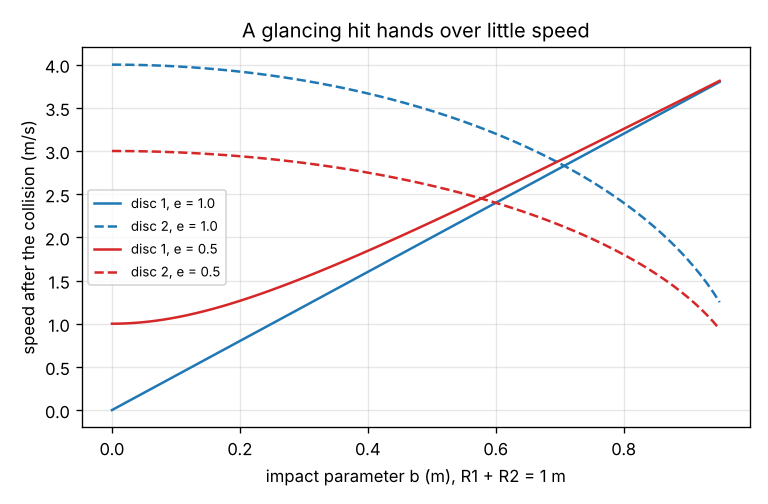
\includegraphics[width=0.78\textwidth]{figures/s03_speeds_vs_impact.png}\caption{Speeds of the two discs after the collision against the impact parameter, for e = 1 and e = 0.5.}\end{figure}

\begin{figure}[h]\centering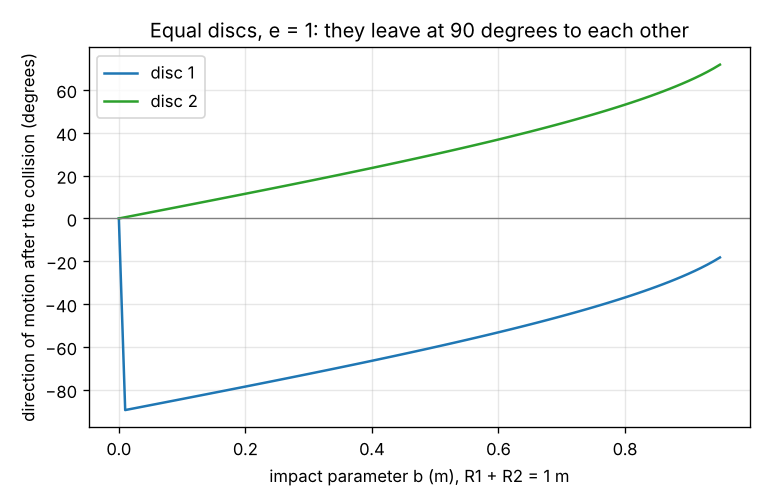
\includegraphics[width=0.78\textwidth]{figures/s03_angles_vs_impact.png}\caption{Direction of each disc after the collision, for equal masses and e = 1.}\end{figure}

\subsection*{E. Worked example}
\textbf{Problem.} Disc 1 (1 kg, radius 0.5 m) moves at 4 m/s along +x and hits disc 2 (1 kg, radius 0.5 m) at rest. The impact parameter is b = 0.5 m and e = 1. Find both velocities after the collision.

\begin{enumerate}[nosep]
\item sin(phi) = 0.5 / 1.0, so phi = 30 degrees and n = (0.866, 0.5).
\item v\_n = (4, 0) . n = 3.464 m/s.
\item v1' = (4, 0) - (1/2) x 2 x 3.464 x n = (1.00, -1.73) m/s: speed 2.00 m/s at -60 degrees.
\item v2' = 0 + (1/2) x 2 x 3.464 x n = (3.00, 1.73) m/s: speed 3.46 m/s at 30 degrees.
\item Check momentum: (1.00 + 3.00, -1.73 + 1.73) = (4, 0), the same as before.
\item Check energy: 1/2 x 1 x 4 + 1/2 x 1 x 12 = 8 J = 8 J before.
\item Check the angle: (1.00, -1.73) . (3.00, 1.73) = 0, so the discs leave at 90 degrees to each other.
\end{enumerate}
\textbf{Answer.} Disc 1: (1.00, -1.73) m/s. Disc 2: (3.00, 1.73) m/s. The angle between them is 90 degrees.

\section*{Where to go next}
\begin{enumerate}[nosep]
\item \textbf{Friction and spin between discs.} Add a friction impulse along the contact surface (Coulomb friction with a given coefficient) and a spin for each disc.
\item \textbf{Many bodies: Newton's cradle.} A time-stepping simulation of five equal balls in a row with a restitution coefficient, using the Session 2 rule for every contact.
\item \textbf{Rotating bodies and angular momentum.} A collision of a point mass with a free rod, using conservation of linear and angular momentum.
\item \textbf{A better crumple zone.} Replace the constant average force of Session 3 by a force that grows linearly with the crumple distance, and compute the peak force and the stopping distance.
\item \textbf{A ball bouncing in a box.} A ball bouncing on a floor with restitution e, with the time and speed of every bounce computed exactly.
\end{enumerate}

This is a simplified educational model. It is not a validated design tool and must not be used for real structures, electrical installations, vehicles, industrial processes or medical decisions.

\end{document}
